\documentclass[conference]{IEEEtran}
\IEEEoverridecommandlockouts
% The preceding line is only needed to identify funding in the first footnote. If that is unneeded, please comment it out.
\usepackage{cite}
\usepackage{amsmath,amssymb,amsfonts}
\usepackage{algorithmic}
\usepackage{graphicx}
\usepackage{textcomp}
\usepackage{xcolor}
\usepackage{float}
\def\BibTeX{{\rm B\kern-.05em{\sc i\kern-.025em b}\kern-.08em
    T\kern-.1667em\lower.7ex\hbox{E}\kern-.125emX}}
\begin{document}

\title{Sentiment Analysis on Twitter Using Machine Learning\\
%{\footnotesize \textsuperscript{*}Note: Sub-titles are not captured in Xplore and
%should not be used}
%\thanks{Identify applicable funding agency here. If none, delete this.}
}

\author{\IEEEauthorblockN{1\textsuperscript{st} Amardeep Singh Dhillon}
\IEEEauthorblockA{\textit{Department of Mathematics and Computing} \\
\textit{Mount Royal University}\\
Calgary, Canada \\
adhil365@mtroyal.ca , ORCID:0009-0009-7729-3060}
}

\maketitle

\begin{abstract}
This paper presents a sentiment analysis project utilizing the Sentiment140 dataset, which contains 1.6 million labeled Twitter tweets. 
The primary objective is to classify tweets into positive or negative sentiment categories, thereby providing valuable insights into public
 opinion on social media platforms. The dataset underwent extensive preprocessing, including the removal of noisy elements such as URLs, user mentions, 
 and special characters, as well as the expansion of abbreviations and the application of lemmatization for text normalization. Various machine learning models, 
 including Logistic Regression, Support Vector Machines (SVM), and Naïve Bayes, were applied to the task of sentiment classification. Model performance w
 as evaluated using standard metrics, including accuracy, precision, recall, and F1-score. Results indicate that the Logistic Regression model outperformed 
 the others, achieving the highest accuracy. This study contributes to the growing field of sentiment analysis, with potential applications in business i
 ntelligence, social media trend analysis, and public opinion monitoring.
\end{abstract}


\begin{IEEEkeywords}
        Sentiment Analysis, Sentiment140 Dataset, Machine Learning, Logistic Regression, Support Vector Machines, 
        Text Preprocessing, Public Opinion, Social Media, Model Evaluation, Natural Language Processing (NLP)
\end{IEEEkeywords}

\section{Introduction}
Sentiment analysis is the task of determining the sentiment expressed in a piece of text, 
which can be classified as positive, negative, or neutral. With the proliferation of social media platforms such as Twitter, 
analyzing public opinion has become more accessible. Sentiment analysis of Twitter data can be particularly valuable for businesses, 
researchers, and policymakers who want to understand the views and emotions of the public. This project aims to classify tweets as either p
ositive or negative based on their sentiment using the Sentiment140 dataset. This dataset provides a large-scale, labeled collection of tweets, 
making it a popular benchmark for sentiment analysis tasks. However, working with raw Twitter data presents challenges due to its informal nature, 
the presence of slang, and irrelevant content like URLs and user mentions.

\section{Related Work}
Sentiment analysis on social media platforms has been extensively studied, with early research focusing on rule-based methods and lexicon-based approaches 
for sentiment classification. Pang and Lee [1] demonstrated the efficacy of feature-based classifiers, such as Naïve Bayes, for sentiment analysis. T
hese models rely on predefined features such as word frequencies and sentiment lexicons. Over time, more sophisticated machine learning models, including S
upport Vector Machines (SVM), and deep learning models like Long Short-Term Memory (LSTM) networks, have been employed to capture the complex nature of 
social media language. Kim [2] showed that Convolutional Neural Networks (CNNs) could be effectively used for sentiment analysis on short text, such as tweets, 
due to their ability to automatically learn hierarchical features from text. Similarly, Zhou et al. [3] employed deep learning techniques to improve sentiment 
classification on noisy, unstructured data such as Twitter messages, achieving higher accuracy than traditional models.
\\
\\
In recent years, challenges such as sarcasm detection, handling noisy data, and improving model robustness have gained attention, particularly in the context
 of social media platforms like Twitter. These issues, including the identification of contextual sentiment and ambiguity, present significant difficulties i
 n achieving high accuracy in sentiment analysis tasks. These challenges also presented obstacles in our project, which we will discuss further in the results 
 and evaluation section. The importance of preprocessing steps, such as tokenization, lemmatization, and the removal of irrelevant content (URLs, user mentions, 
 hashtags), has been widely emphasized as crucial for improving model performance [4]. Furthermore, recent studies by Gao and Sano [5] suggest that combining machine 
 learning models with human insights in sentiment analysis can improve the accuracy of detecting nuanced expressions such as sarcasm and irony. These preprocessing 
 techniques and challenges were also discussed in our class with Dr. Maryam Elhussein, a professor at Mount Royal University.
 \\
\section{Dataset}
The dataset used in this project is the Sentiment140 dataset, which contains 1.6 million labeled tweets. Each tweet is classified as either positive 
(1) or negative (0) based on its sentiment. The dataset was sourced from Kaggle and provides a broad spectrum of opinions from Twitter users on various topics,
 ensuring a diverse range of linguistic patterns. This dataset was selected for its large size, availability, and its established status as a benchmark in s
 entiment analysis research. However, raw Twitter data presents several challenges, including the presence of URLs, user mentions, hashtags, and informal language. 
 These elements can be noisy and irrelevant to the sentiment classification task, necessitating extensive preprocessing.
\\
\\
As part of the preprocessing process, we renamed the dataset columns to more meaningful labels: 'sentiment', 'ids', 'date', 'flag', 'user', and 'text'. 
The dataset was then encoded using ISO-8859-1 encoding to handle special characters. We also converted sentiment values of 4 to 1, representing positive sentiment, 
and replaced the remaining values with 0, indicating negative sentiment. 
\\
\\
To improve processing efficiency, we removed unnecessary columns and took a 25 percent
fraction of the dataset to reduce its size, as the original dataset was very large. The final dataset, containing only the 'text' and 'sentiment' columns, was 
stored in a list and converted to a Parquet format for faster access. 
\\
\\
To ensure data integrity, we verified the processed dataset by using dataset.head(), 
confirming the accuracy of our preprocessing steps. Finally, the distribution of sentiment labels was checked and found to be evenly split between positive 
and negative tweets, ensuring a balanced dataset for model training.

\section{Methods}
In this study, we employed several machine learning techniques for sentiment classification: Logistic Regression, Support Vector Machines (SVM), and Naïve Bayes. 
These models were selected based on their proven effectiveness in text classification tasks.
 The preprocessing and data cleaning process was essential for ensuring that the raw data was suitable for analysis. 
 To streamline this process, we encapsulated all the cleaning steps into a single function that called several sub-functions. 
 \\ \\ 

 These sub-functions performed various tasks, such as removing HTML tags, URLs, and punctuation, converting text to lowercase, replacing chat abbreviations, 
 removing stopwords, and handling other common issues found in Twitter data. For stopwords, we used the nltk library. 
 Additional functions were used for handling whitespace, special characters, and emojis, as well as expanding common contractions and lemmatizing the text.
  We also loaded SpaCy to assist with text processing tasks.

After performing these cleaning steps, we conducted exploratory data analysis (EDA) to better understand the data. 
One of the first tasks was to generate a word frequency plot of the cleaned data, which revealed that words like “im” and “day” appeared most frequently, 
as shown in Figure A. \\
\begin{figure}[H]
        \centering
        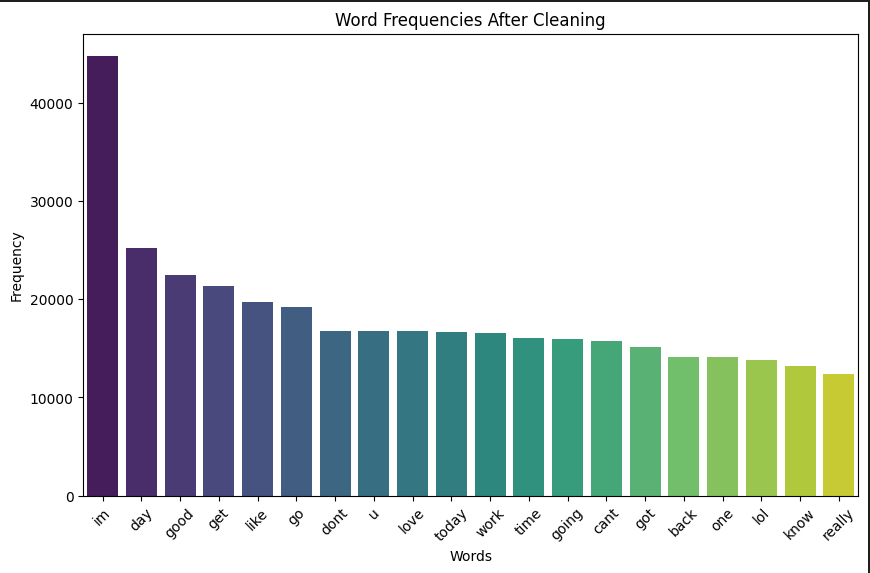
\includegraphics[width=\linewidth]{assets/Word_Freq_Chart.png}
        \caption{Word Frequency Chart}
        \label{fig:word_freq_chart}
    \end{figure}
      
\\
To further analyze sentiment, we created two word clouds: the first represented the most frequent words in positive tweets (Figure B),
 where the word "love" emerged as a dominant theme.
 \begin{figure}[H]
        \centering
        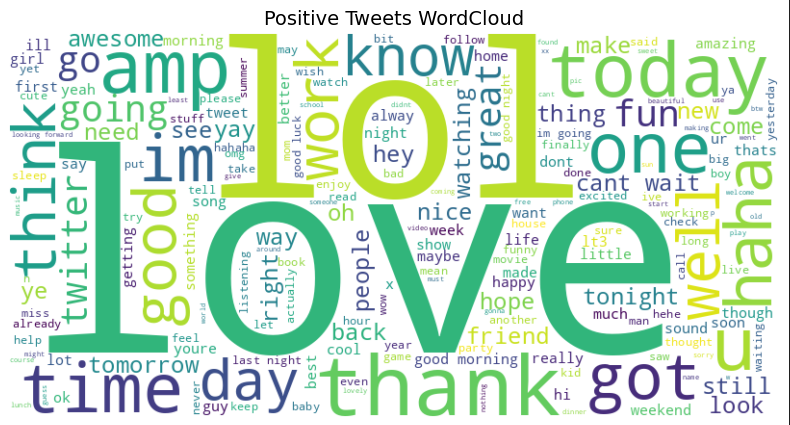
\includegraphics[width=\linewidth]{assets/PositiveWorldCloud.png}
        \caption{Positive Word Cloud}
        \label{fig:PositiveWordCloud}
    \end{figure} 
    \\
    The second word cloud depicted frequent words in negative tweets (Figure C), where the word "today" stood out. 
 These visualizations provided useful insights into the linguistic patterns present in positive and negative sentiments.
 \begin{figure}[H]
        \centering
        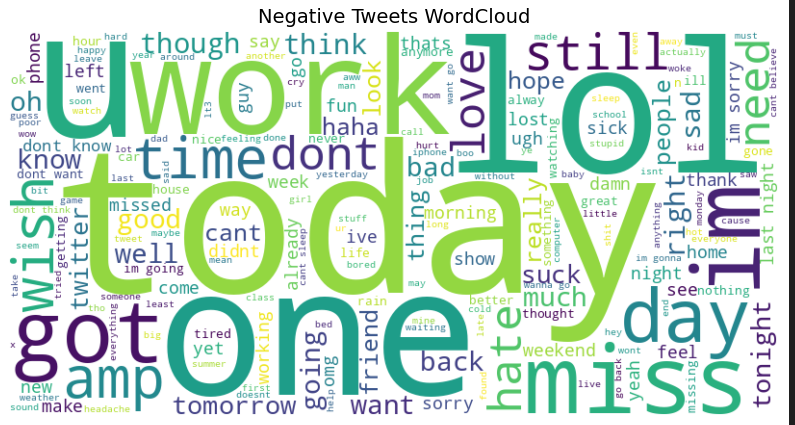
\includegraphics[width=\linewidth]{assets/NegativeWordCloud.png}
        \caption{Negative Word Cloud}
        \label{fig:NegativeWordCloud}
    \end{figure}
 \\
\section{Results and Evaluation}
Before training the machine learning models, we converted the tokenized text into Bag of Words features. 
The dataset was split into an 80-20 training-to-testing ratio, with a random state of 42 to ensure reproducibility. 
We limited the maximum number of features to 5000 to reduce dimensionality and enhance model efficiency. 
The performance of the models was evaluated based on standard classification metrics: accuracy, precision, recall, and F1-score. 
The results for these metrics, along with the confusion matrices, are provided in the attached figures. 
The confusion matrices have been visualized in heatmaps and we will only provide the heatmap for Logistic Regression for better interpretation.
\begin{figure}[H]
        \centering
        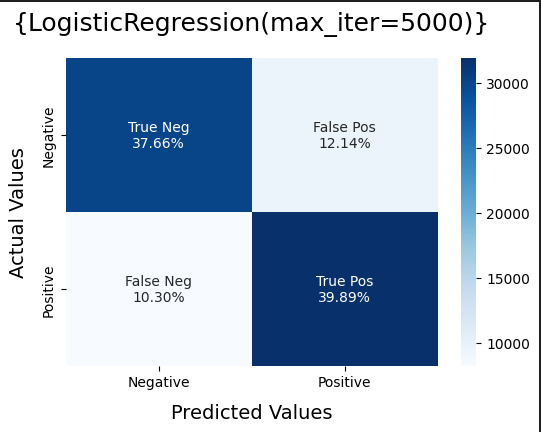
\includegraphics[width=\linewidth]{assets/LR_ConfusionMatrix.png}
        \caption{Logistic Regression Confusion Matrix}
        \label{fig:Logistic_Regression_Confusion_Matrix}
    \end{figure}

For accuracy, the performance of the models was as follows: Logistic Regression achieved an accuracy of 77.55, 
Naïve Bayes scored 76.52, and Support Vector Classifier (SVC) scored 75.93. These results indicate that all three models performed relatively well, 
with Logistic Regression slightly outperforming the others. To evaluate the best-performing model, we saved it using pickle and later reloaded it for further analysis. 
Using the glob library, we located the saved model file, and through the command line, we input text, which was classified as either positive or 
negative sentiment.
\\
\\
However, one significant limitation we encountered during the evaluation process was the inability of the models to accurately handle sarcasm in the tweets. 
This was evident in our tests, where sarcastic remarks were misclassified, reflecting the ongoing challenge of detecting sarcasm in sentiment analysis tasks.
\section{conclusion}
This project demonstrated the application of machine learning models to classify sentiment in Twitter tweets. The Logistic Regression model proved to be the 
most effective in classifying the sentiment, providing better accuracy and recall than Logistic Regression. The key preprocessing steps—such as 
lemmatization, URL removal, and emoji handling—were crucial in improving the models' performance. Despite these improvements, challenges remain, 
particularly in detecting sarcasm and understanding the context of tweets, which are crucial for improving sentiment analysis. Future work could 
explore the use of deep learning models, such as BiLSTM, and tackle the problem of handling sarcasm and nuanced expressions in tweets. The findings
 have real-world applications in understanding public sentiment on social media platforms, with potential uses in business, politics, and social 
 research.
\section*{References}
Pang, B., & Lee, L. (2004). Thumbs up? Sentiment classification using machine learning techniques. 
Proceedings of the ACL-2004 Conference on Empirical Methods in Natural Language Processing, 79–86. 
\\
\\
Yoon Kim. 2014. Convolutional Neural Networks for Sentence Classification. In Proceedings of the 2014 Conference on Empirical Methods in Natural 
Language Processing (EMNLP), pages 1746–1751, Doha, Qatar. Association for Computational Linguistics
\\
\\
Zhou, P., Huang, Z., & Zhao, L. (2016). Deep learning for sentiment analysis of short texts with noise.
 Proceedings of the 2016 Conference on Empirical Methods in Natural Language Processing, 2357–2363.
 \\
 \\
 Liu, B., & Zhang, L. (2012). A survey of opinion mining and sentiment analysis.
  In Mining Text Data (pp. 415–463). Springer.
  \\
  \\
  Gao, Q., & Sano, T. (2019). Combining machine learning models with human insights 
  for sentiment analysis. Proceedings of the 2019 IEEE International Conference on Data Mining Workshops, 123–130.
%\begin{thebibliography}{00}
%\bibitem
%\end{thebibliography}
\vspace{12pt}

\end{document}
